\documentclass[utf8]{beamer}

\title{Lounge-o-Matic\\{\small \textit{A private streaming service.}}}
\author{Axel Sundbom\\Ravilj Adelbrun}

\begin{document}

\begin{frame}
\maketitle
\end{frame}

\begin{frame}
\frametitle{Technical Choices}

\begin{columns}
	\begin{column}{0.6\textwidth}
		\begin{itemize}
			\item Frontend-backend architecture
			\item Full-stack Flask
			\item RESTful API
			\item WebSocket streaming
			\item NGINX reverse proxy and load-balancer
			\item MySQL database storage
		\end{itemize}
	\end{column}

	\begin{column}{0.4\textwidth}
		\includegraphics[width=\textwidth]{img/flask-logo.png}
	\end{column}
\end{columns}
\end{frame}

\begin{frame}
\frametitle{Project Direction}

\begin{itemize}
	\item Seven-day agile sprints
	\item Varying amount of time available
	\item Yodiz backlog manager
	\item Frontend/backend work-division\\with ``seminar'' sessions
\end{itemize}
\end{frame}

\begin{frame}
\frametitle{Current Status}
\begin{columns}
	\begin{column}{0.6\textwidth}
	\begin{itemize}
		\item Research stage mostly completed
		\item API samples communicate with database
		\item Rough draft of database schema finished
	\end{itemize}
	\end{column}

	\begin{column}{0.4\textwidth}
		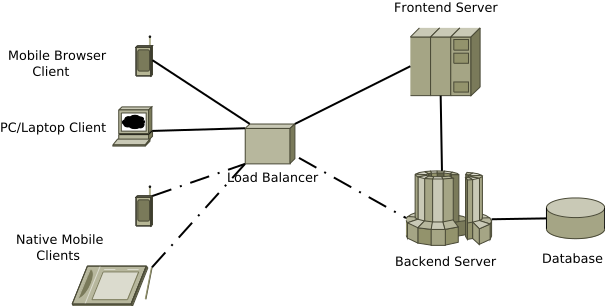
\includegraphics[width=\textwidth]{img/arch.pdf}
	\end{column}
\end{columns}
\end{frame}

\end{document}
